\documentclass[30pt,twocolumn,letterpaper]{article}
\usepackage{cvpr}
\usepackage{times}
\usepackage{booktabs}
\usepackage{epsfig}
\usepackage{graphicx}
\usepackage{amsmath}
\usepackage{amssymb}
\cvprfinalcopy
\def\cvprPaperID{****}
\def\httilde{\mbox{\tt\raisebox{-.5ex}{\symbol{126}}}}
\usepackage{graphicx}
\usepackage{indentfirst}
\setlength{\parindent}{2em}
\usepackage{cite}
\usepackage[colorlinks,linkcolor=red,anchorcolor=blue,citecolor=green,backref=page]{hyperref}
\author{Qilei Zhang\\\\
Jun 12 2018}
\title{Decoupled Neural Interfaces Using Synthetic Gradients}
\begin{document}
\maketitle
\begin{abstract}
  Training directed neural networks typically requires forward-propagating data through a computation graph, followed by backpropagating error signal, to produce weight updates.
\end{abstract}
\section{Introduction}
Each layer (or module) in a directed neural network can be considered a computation step, that transforms its incoming data. These modules are connected via directed edges, creating a forward processing graph which defines the flow of data from the network inputs, through each module, producing network outputs\cite{Barat2016String}. \\
\begin{figure}[htbp]
\small
\centering
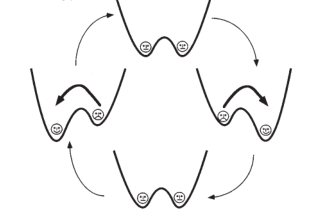
\includegraphics[width=20em]{000.png}
\caption{Transfer ratios on the Amazon benchmark. Both SDA-based systems outperforms the rest, and SDAsh (unsupervised training on all domains) is best.Reproduced from Glorot et al. (2011b).}
\label{fig:lable}
\end{figure}\\
\begin{equation}
\quad x'(t)=-V'(x)+A_0cos(wt+o)+u(t)
\end{equation}
\section{Decoupled Neural Interfaces}
We begin by describing the high-level communication protocol that is used to allow asynchronously learning agents to communicate\cite{Eiber2013Attaining}.\\
\section{Synthetic Gradient for Recurrent Networks}
We begin by describing how our method of using synthetic gradients applies in the case of recurrent networks; in some ways this is simpler to reason about than feed-forward networks or more general graphs\cite{Liu2005Aeroengine}.
\section{Arbitrary Network Graphs}
Although we have explicitly described the application of DNIs for communication between layers in feed-forward networks\cite{Mahendran2015Visualizing}, and between recurrent cores in recurrent networks, there is nothing to restrict the use of DNIs for arbitrary network graphs\cite{Yi2010Effective}.
{\small
\bibliographystyle{ieee}
\bibliography{1}
}
\end{document}
